% id: 64-23
% book: 쎈B 대수 · 05 삼각함수
% section: 유형 06 부채꼴의 호의 길이와 넓이
% figure: tikz:fig-64-23
% answer: 
% answer_source: 
% variant_level: 0 (원본 전사)
% 이 파일은 build.mjs 가 items.json 에서 만든다. 고칠 때는 items.json 을 고친다.
\noindent\begin{minipage}[t]{0.58\linewidth}\vspace{0pt}\raggedright 오른쪽 그림과 같이 길이가 $12$인 선분~$\pt{AB}$를 지름으로 하는 반원이 있다. 반원 위에서 호 $\pt{AC}$의 길이가 $4\pi$인 점~$\pt{C}$를 잡고 점~$\pt{C}$에서 선분~$\pt{AB}$에 내린 수선의 발을 $\pt{H}$라 하자. 이때 색칠한 부분의 넓이를 구하시오.\end{minipage}\hfill\begin{minipage}[t]{0.4\linewidth}\vspace{0pt}\centering \resizebox{\ifdim\width>\linewidth\linewidth\else\width\fi}{!}{% 64-23(64쪽) — 지름 AB 의 길이가 12 인 반원, 호 AC 의 길이가 4π 인 점 C 와 C 에서 AB 에 내린 수선의 발 H, 색칠한 부분.
% 스캔 화질이 낮아 TikZ 로 다시 그림. 원문 그림의 표시(A · B · C · H · 12 · 직각 기호)만 둔다.
% 색칠한 부분의 넓이(답)는 그림에 적지 않는다.
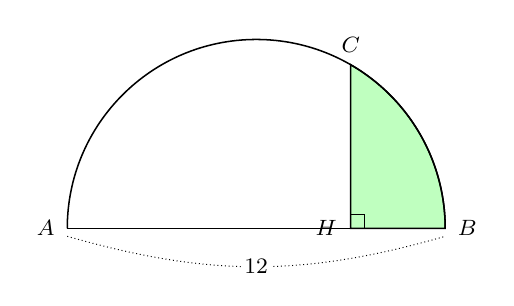
\begin{tikzpicture}[scale=0.4, line width=0.55pt, >=stealth]
  \filldraw[fill=green!25] (3,0) -- (6,0) arc (0:60:6) -- cycle;
  \draw (-6,0) arc (180:0:6);
  \draw (-6,0) -- (6,0);
  \draw[line width=0.35pt] (3,0.45) -- (3.45,0.45) -- (3.45,0);
  \draw[densely dotted, line width=0.35pt] (-6,-0.25) to[bend right=16] node[midway, fill=white, inner sep=1pt, font=\footnotesize] {$12$} (6,-0.25);
  \node[left=1pt, font=\footnotesize] at (-6,0) {$\pt{A}$};
  \node[right=1pt, font=\footnotesize] at (6,0) {$\pt{B}$};
  \node[above=1pt, font=\footnotesize] at (60:6) {$\pt{C}$};
  \node[left=1.5pt, font=\footnotesize] at (3,0) {$\pt{H}$};
\end{tikzpicture}
}\end{minipage}\par
